A first approach to solve this problem was presented in Ramsay and Silverman
(2005) \cite{Ramsay2005}, by considering a simple shift in the domain to make the
registration. Although it is a basic approach, it will be useful in many cases.
Figure \ref{SBFIG:SHIFT1} shows a set of sinusoidal waves whose phases are not
aligned, and a shift in the time scale will be adequate to make the alignment.

Let $\{x_i\}_{i=1}^n$ be a set of functional observations, which will be aligned
using this transformation. We are actually interested in finding the values

\begin{equation}[EQN:SHIFTS]{Shift registrtion}
x_i^*(t)=x_i(t+ \delta_i) \qquad i=1,2, \dots n
\end{equation}

where the shift parameter $\delta_i$ is chosen in order to align the features of
the curves. In the figure \ref{SBFIG:SHIFT2} it is shown the result of apply
this type of transformation to the set of sinusoidal waves.


A possible solution for the calculation of shifts $\delta_i$, is using a least
square criterion, minimizing the registered sum of squared errors (REGSSE),
defined as

\begin{equation}[EQ:REGSSE]{Least square criterion}
\text{REGSSE} = \sum_{i=1}^{n}\int_{\mathcal{T}}\left [x_i(t+\delta_i) - \hat \mu(t) \right ]^2 dt
\end{equation}

The alignment problem will be based on finding the values $\delta_i$ that
minimize this sum of errors. For this purpose,
we will use the derivatives of the functions $x_i$, using a variant of the
Newton-Rhapson method. A description of the algorithm used to calculate these
values is given in the Appendix \ref{SEC:NEWTON}.

\begin{figure}[Shift registration of a dataset]{FIG:SHIFT}{Shift registration of a dataset}
	\subfigure[SBFIG:SHIFT1]{Unregistered curves $x(t)$}{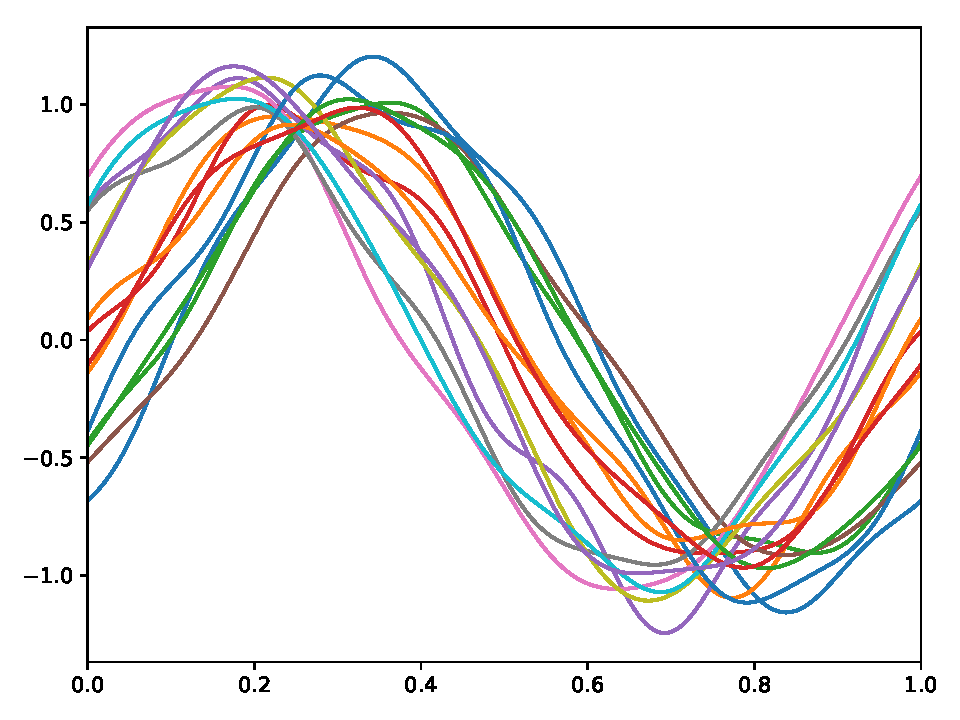
\includegraphics[width=7.5cm]{sine-waves}} \quad
	\subfigure[SBFIG:SHIFT2]{Registered curves $x^*(t)$}{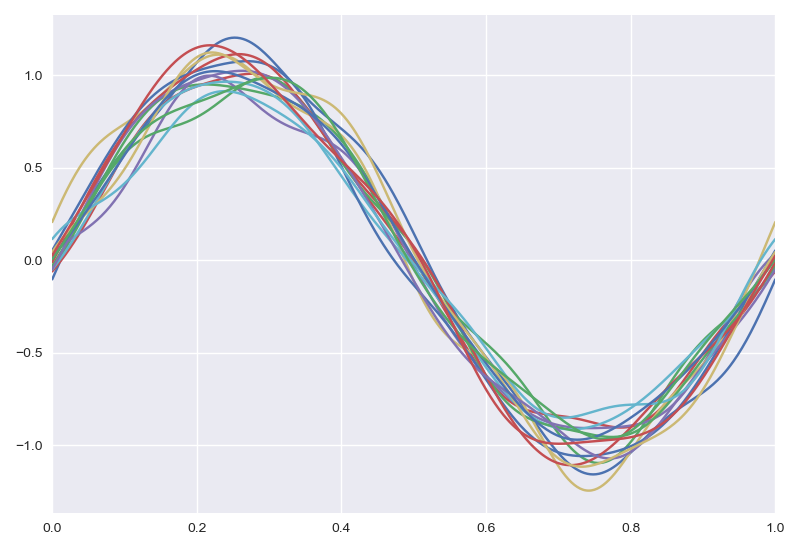
\includegraphics[width=7.5cm]{sine-waves-shifted}}
\end{figure}
